\documentclass[12pt, letter paper]{report}
\usepackage{graphicx} % Required for inserting images
\usepackage[document]{ragged2e}
\usepackage[a4paper, total={6in, 7in}]{geometry}
\setcounter{tocdepth}{6} 
\setcounter{secnumdepth}{6} 
\setcounter{chapter}{0}
\usepackage{blindtext}
\usepackage{layout}
\usepackage[dvipsnames]{xcolor}
\usepackage{biblatex} %Imports biblatex package
\addbibresource{sample.bib} %Import the bibliography file
\usepackage{geometry}
\usepackage{hyperref}


 \geometry{
 a4paper,
 total={170mm,257mm},
 left=27mm,
 top=20mm,
 }


\title{DBMS MINIPROJECT REPORT }
\author{Darren Pereira}
\date{August 2023}

\begin{document}
\thispagestyle{empty}
%\maketitle
%cover page 
\begin{center}
\Large\textbf{ ST JOSEPH ENGINEERING COLLEGE\\ }
\textbf{An Autonomous Institution}\\
Affiliated to VTU, Belagavi\\
\textbf{Mangaluru-575028}
\end{center}

\begin{figure}[h]
 \centering
 
\includegraphics[scale=1.1]{sjec.jpeg}
 \label{sjeclogo}
\end{figure}

\begin{center}
   \textbf{ MINI PROJECT REPORT ON }
\end{center}
\begin{center}
   \Large\textbf{“PHARMACY DATABASE MANAGEMENT”}
\end{center}



 
\begin{center}
   \Large \textbf{Submitted By \\}
\end{center}

\begin{center}
\justifying{
Darren Pereira\hspace{9.5 cm}4SO21CS042\\

}
\justifying{

\hspace{-0.6 cm}Karthik Nayak\hspace{9.5 cm}4SO21CS058\\
}
\justifying{
	
\hspace{-0.6 cm}Clancy Dsouza\hspace{9.5 cm}4SO21CS040\\
}
\end{center}
   \begin{center}
\large \textbf{\\Under the guidance of \\}
\large  \textbf{ \\Ms Pruthvi M R\\ }
\large  Assistant Professor,\\ Department of CSE
\end{center}

\vspace{0.5cm}
\begin{center}
\large\textbf{\\ DEPARTMENT OF COMPUTER SCIENCE AND ENGINEERING\\ 2022-2023}

\end{center}
\vspace{2cm}
\thispagestyle{empty}
% certificate Page 
\section*{}
\begin{center}
\Large\textbf{\\ ST JOSEPH ENGINEERING COLLEGE}\\
\end{center}
\begin{center}
\textbf{\textit{An Autonomous Institution}}\\

\large \textbf{Vamanjoor, Mangaluru-575028}\\
\large \textbf{ DEPARTMENT OF COMPUTER SCIENCE AND ENGINEERING} 
\end{center}
\vspace{0.1cm}
\begin{center}
\begin{figure}[h]
 \centering
 
\includegraphics[scale=0.7]{sjec.jpeg}
 \label{sjeclogo}
\end{figure}
\end{center}
\vspace{-1cm}
\begin{center}
\large\textbf{\textcolor{blue}{CERTIFICATE}}
\end{center}
\begin{center}
\justifying{
\large Certified that the project work entitled \textbf{“Pharmacy Management System”} carried out by }
\end{center}
\begin{center}
\justifying{
\hspace{3.5 cm}Darren Pereira\hspace{4.35 cm}4SO21CS042
}
\end{center}
\begin{center}
\justifying{
\hspace{3.5 cm}Karthik Nayak\hspace{4.35 cm}4SO21CS058
}
\end{center}
\begin{center}
\justifying{
\hspace{3.5 cm}Clancy Dsouza\hspace{4.35 cm}4SO21CS040
	}
\end{center}

\begin{center}
\justifying{
\par{

\large bonafide students of IV semester students in partial fulfillment for the award of Bachelor of Engineering in Computer Science and Engineering of St Joseph Engineering College during the year 2022-23.It is certified that all corrections/\\suggestions indicated during Internal Evaluation have been incorporated in the report.The project report has been approved as it satisfies the academic requirements in respect of miniproject work .\\\\\\

} 
}
\end{center}
\begin{center}
\justifying{ 
\large\textbf{Ms Pruthiv M R \hspace{7.3 cm}  Dr Sridevi Saralaya  \\}
\hspace{1cm}\large\textbf{  Project Guide \hspace{8 cm} HOD-CSE 
}
}

\end{center}
\begin{center}
  
\large\textbf{ \\EXTERNAL VIVA}
\end{center}
\justifying{ 
\large\textbf{
NAME OF THE EXAMINER  \hspace{4 cm}  SIGNATURE \\\\ 1.\\\\2.}}

\thispagestyle{empty}
\newpage
\chapter*{\centering Acknowledgment}
\justifying{
\addcontentsline{toc}{chapter}{\numberline{}Acknowledgment}
% \linespread
  \large The satisfaction and euphoria that accompanies the successful completion of any task would be incomplete without mentioning the people who made it possible, whose constant guidance and encouragement crowned our efforts with success.\\
    \\
    We take this opportunity to thank those who have helped and motivated us throughout the completion of this project.\\
    \\
    We would like to express our deep and sincere gratitude to our project guide,\textbf{Ms Pruthvi M R}, Assistant Professor, Department of Computer Science and Engineering, for her constant guidance and support, without which this project wouldn’t have been completed successfully. \\
    \\ 
    We owe our great debt to \textbf{Dr Sridevi Saralaya}, Head of the Department of Computer Science and Engineering, for her support and encouragement during the course of development of this project. \\
    \\
    We are immensely grateful to our Principal, \textbf{Dr Rio D’Souza}, our Director, \textbf{Rev. Fr Wilfred Prakash D’Souza}, and Assistant Director \textbf{Rev. Fr Kenneth Rayner Crasta} for their support and encouragement. \\
    \\
    We extend our gratitude to the entire faculty and the staff of the Department of Computer Science and Engineering, SJEC, for their advice, kind co-operation and assistance throughout the academic year.\\
    \\
    Lastly, we would like to express our heartfelt appreciation towards our classmates and seniors for their guidance and suggestions.
 
    
 }
%/\thispagestyle{empty}
\pagenumbering{roman}
\chapter*{\centering Abstract}

\justifying{
\addcontentsline{toc}{chapter}{\numberline{}Abstract}
The main aim of the project is the management of the database of the pharmaceutical shop. This project is insight into the design and implementation of a Pharmacy Management System. This is done by creating a database of the available medicines in the shop. The primary aim of pharmacy management system is to improve accuracy and enhance safety and efficiency in the pharmaceutical store. The aim of this project is to develop software for the effective management of a pharmaceutical store. We have developed this software for ensuring effective policing by providing statistics of the drugs in stock.\\
\\
This program can be used in any pharmaceutical shops having a database to maintain it. The software used can generate reports, as per the user’s requirements. The software can print invoices, bills, receipts etc. It can also maintain the record of supplies sent in by the supplier. Here, the admin who are handling the organization will be responsible to manage the record of the employee. Each employee will be given with a separate username and password. \\
\\
The aim of the project is to create an effective software to help the pharmacist to maintain the records of the medicines, handle user details, generate invoice, check and renew validity and provide a scope of communication between users by using inbuilt messaging system. Pharmacy management system deals with the maintenance of drugs and consumables in the pharmacy unit. This pharmacy management system is user friendly. \\
\\

}
%/\thispagestyle{empty}



%\section*{\centering TABLE OF CONTENT}
%/\thispagestyle{empty}
\renewcommand{\contentsname}{Table of Contents}
\tableofcontents
\addcontentsline{toc}{chapter}{\numberline{}Table of Contents}
\listoffigures
\addcontentsline{toc}{chapter}{\numberline{}List of Figures}
\listoftables
\addcontentsline{toc}{chapter}{\numberline{}List of Tables}
\newpage
%/\tableofcontents
\thispagestyle{empty}

\chapter{Introduction}
The project's primary objective is to streamline pharmaceutical shop database management through the development of a Pharmacy Management System. This system ensures precise medication tracking, bolstering safety and operational efficiency within the store. Our software enables effective stock control, report generation, and secure user access, facilitating seamless interaction between users via an integrated messaging system. It addresses the complex demands of pharmacy management, catering to both administrative and employee needs, offering a user-friendly solution for pharmaceutical establishments.
\section{Problem Definition} 
The problem at hand involves the need for an efficient software solution to aid pharmacists in effectively managing medication records, user information, invoice generation, validity checks, and fostering communication among users within a pharmacy unit. This challenge necessitates the development of a user-friendly Pharmacy Management System capable of handling intricate pharmacy operations and catering to administrative and employee requirements, ultimately enhancing overall pharmacy management.
%\subsection{vvv}
\section{Scope and Importance}
The scope of this Pharmacy Management System encompasses comprehensive medication tracking, user management, invoicing, and communication features, serving pharmaceutical stores of various sizes. Its significance lies in improving accuracy, safety, and efficiency in pharmaceutical operations, reducing errors, enhancing customer service, and enabling better stock control. This system caters to the evolving needs of the pharmacy industry, contributing to its modernization and growth.
\pagenumbering{arabic}
\chapter{Software Requirement Specification}

\section{Description on Implementation} 
List of modules
\begin{itemize}
	
\item Login page
\item Homepage
\item Company
\item Purchase
\item Drugs
\item Sales
\item User/Settings
\item Messaging
\end{itemize}
\section{Software Requirement Specification}
Software Requirement Specification
\begin{itemize}
 \item {\textbf{Language} : Java}
 \item {\textbf{Database used}: MySQL}.
 \item {\textbf{Design used}: Java}.
 \item {\textbf{Operating System}: Window 11}.
 \item {\textbf{Software used}: XAMPP}.
\end{itemize}

\section{Hardware Requirement Specification} 

\begin{itemize}
 \item {\textbf{Installed Memory} : 2GB or Higher}
 \item {\textbf{Processor}: 1GHz or Higher}.
 \item {\textbf{Hard Disk Space}: 16GB availability }.
 \item {\textbf{Display}: Standard outpout display}.
 \
\end{itemize}
\chapter{System Design}
\section{ER Diagram} 
Figure:\ref{fig:er-diagram-for-student-management-system.png} shows the ER diagram of student database.
\begin{figure}[h]
 \centering
 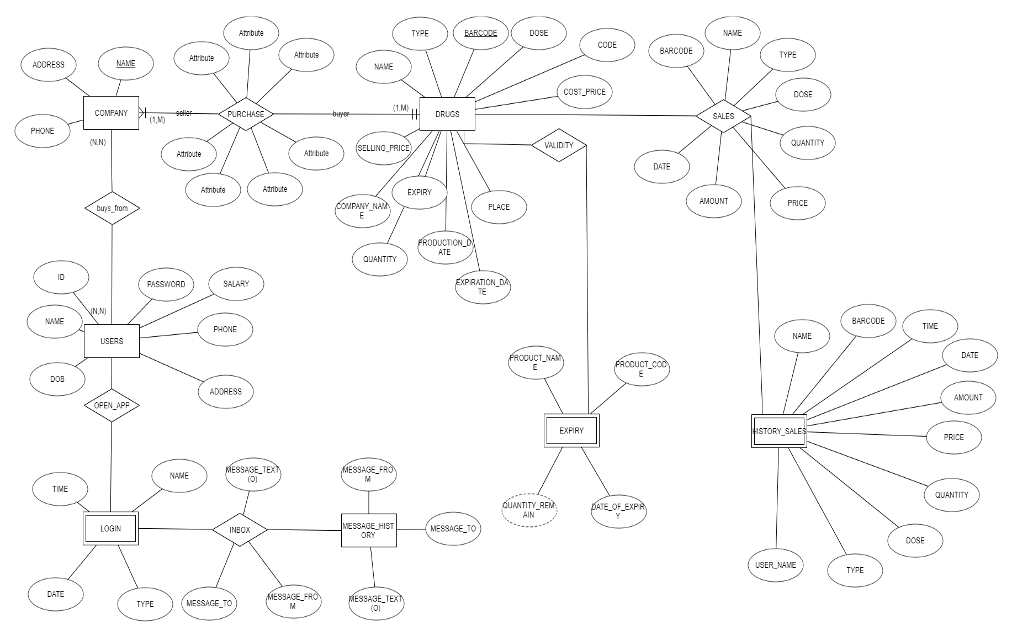
\includegraphics[width=1\textwidth]{er-diagram-for-student-management-system.png}
 \caption{ER diagram}
 \label{fig:er-diagram-for-student-management-system.png}
\end{figure}
\\
\\
\\
\pagebreak
\section{Schema Diagram} 
Figure:\ref{fig:DBMS-Schema.png} shows the Schema Diagram of student Database.
\begin{figure}[h]
 \centering
 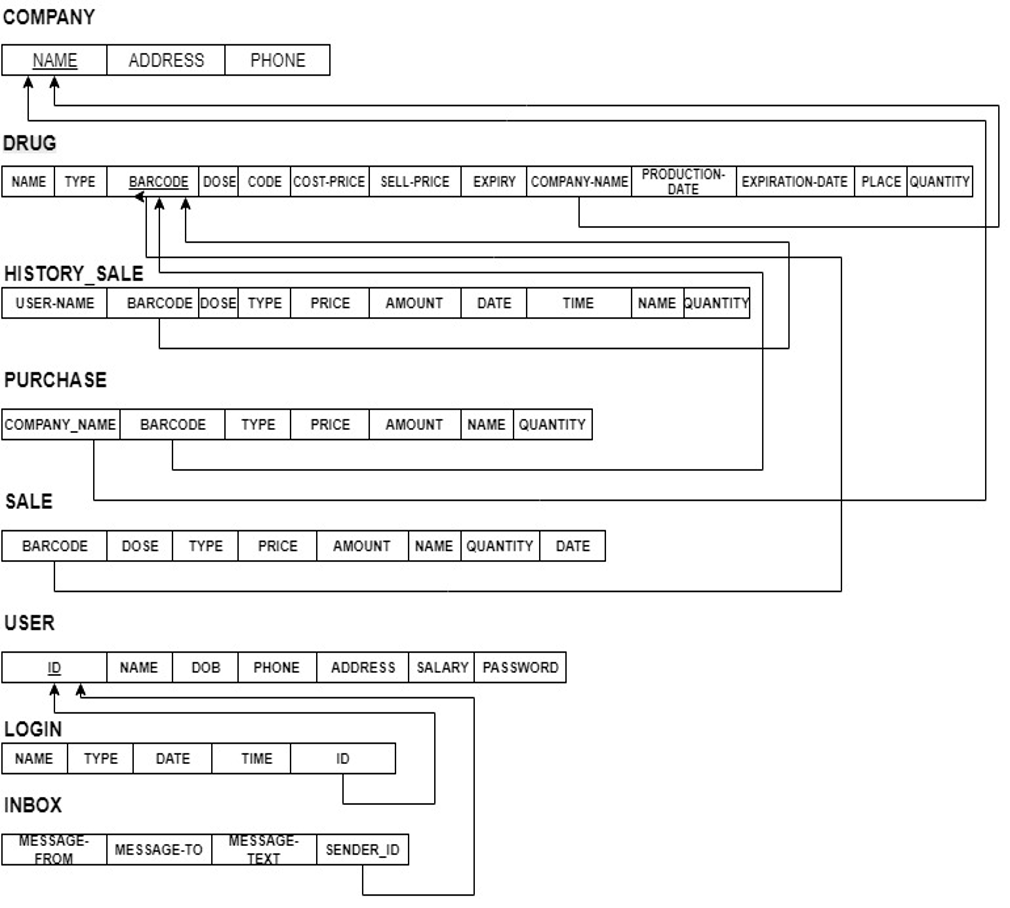
\includegraphics[width=1\textwidth]{DBMS-Schema.png}
 \caption{Schema diagram}
 \label{fig:DBMS-Schema.png}
\end{figure}
\\
\pagebreak
\section{Table description} 
\begin{center}
Table:\ref{table:company.png} 
\begin{table}[h]
	\centering
	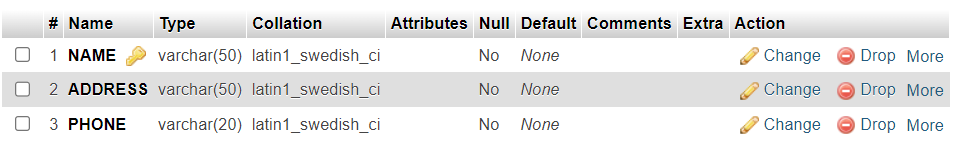
\includegraphics[width=1\textwidth]{company.png}
	\caption{company table}
	\label{table:company.png}
\end{table}
\end{center}

\begin{center}
	Table:\ref{table:drugs.png} 
	\begin{table}[h]
		\centering
		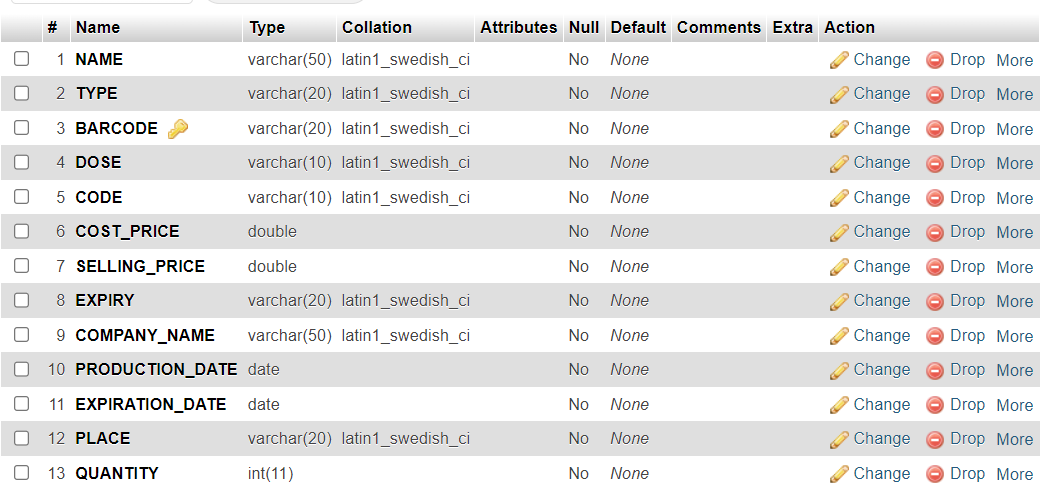
\includegraphics[width=1\textwidth]{drugs.png}
		\caption{drugs table}
		\label{table:drugs.png}
	\end{table}
\end{center}

\begin{center}
	Table:\ref{table:expiry.png}
	\begin{table}[h]
		\centering
		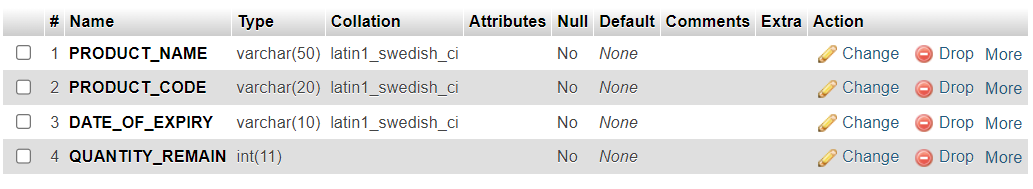
\includegraphics[width=1\textwidth]{expiry.png}
		\caption{expiry table}
		\label{table:expiry.png}
	\end{table}
\end{center}
\newpage
\begin{center}
	Table:\ref{table:history.png}
	\begin{table}[h]
		\centering
		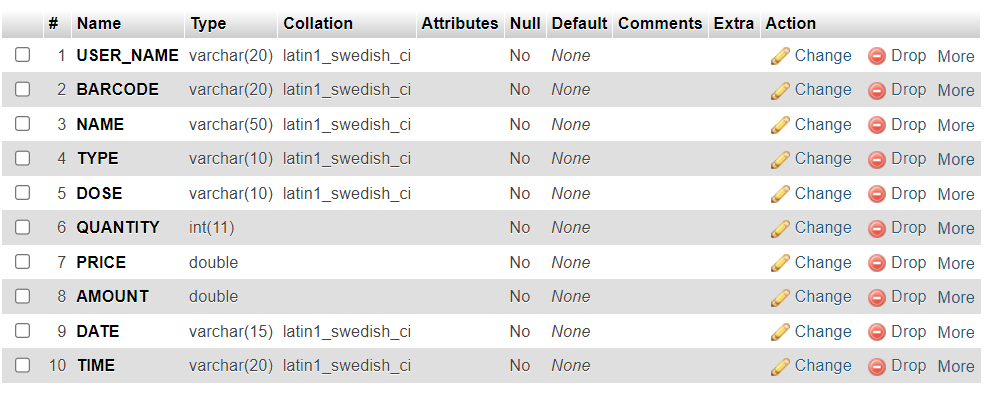
\includegraphics[width=1\textwidth]{history.png}
		\caption{history of sales table}
		\label{table:history.png}
	\end{table}
\end{center}

\begin{center}
	Table:\ref{table:inbox.png}
	\begin{table}[h]
		\centering
		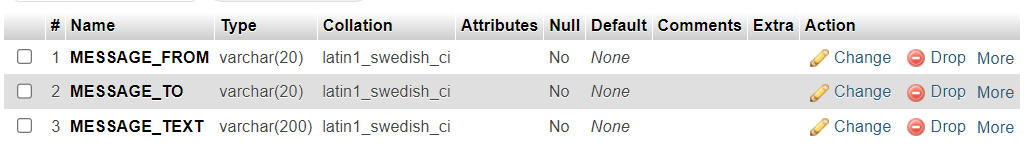
\includegraphics[width=1\textwidth]{inbox.png}
		\caption{inbox table}
		\label{table:inbox.png}
	\end{table}
\end{center}

\begin{center}
	Table:\ref{table:login.png}
	\begin{table}[h]
		\centering
		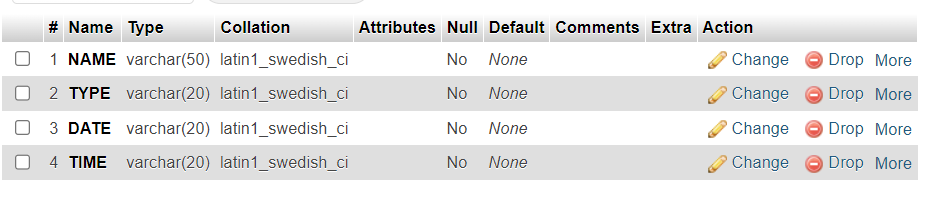
\includegraphics[width=1\textwidth]{login.png}
		\caption{login table}
		\label{table:login.png}
	\end{table}
\end{center}
\newpage
\begin{center}
	Table:\ref{table:messagehist}
	\begin{table}[h]
		\centering
		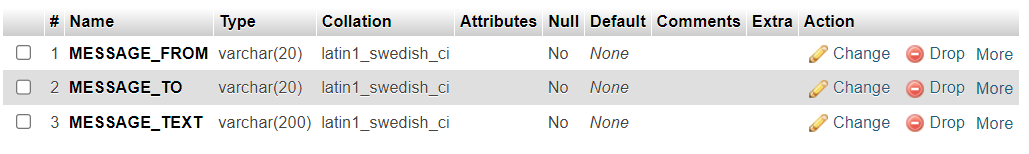
\includegraphics[width=1\textwidth]{messagehist.png}
		\caption{message history table}
		\label{table:messagehist}
	\end{table}
\end{center}

\begin{center}
	Table:\ref{table:purchase.png}
	\begin{table}[h]
		\centering
		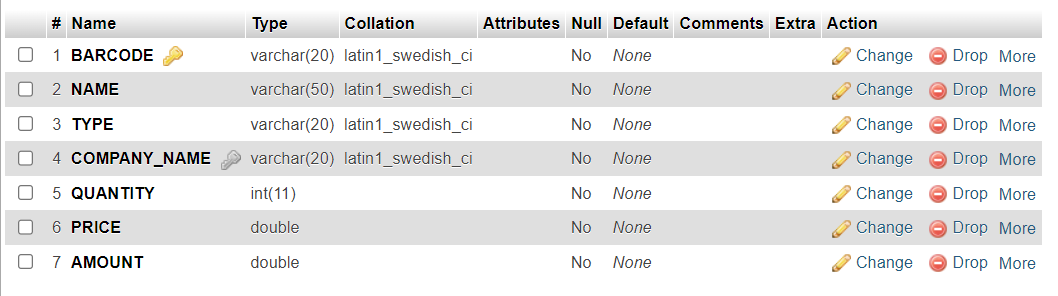
\includegraphics[width=1\textwidth]{purchase.png}
		\caption{purchase table}
		\label{table:purchase.png}
	\end{table}
\end{center}

\begin{center}
	Table:\ref{table:sales.png}
	\begin{table}[h]
		\centering
		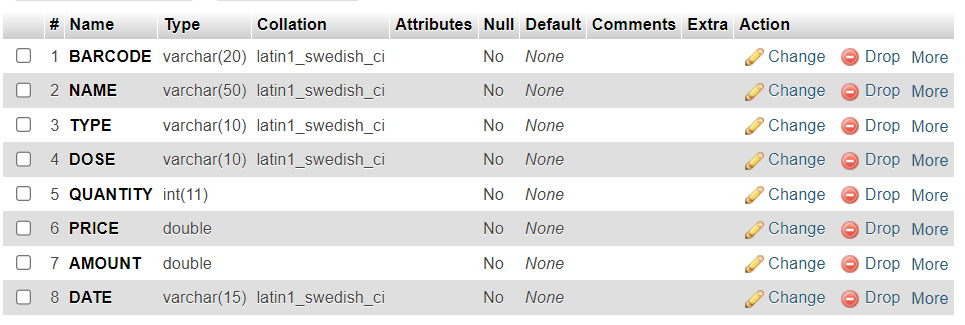
\includegraphics[width=1\textwidth]{sales.png}
		\caption{sales table}
		\label{table:sales.png}
	\end{table}
\end{center}
\newpage
\begin{center}
	table:\ref{table:users.png}
	\begin{table}[h]
		\centering
		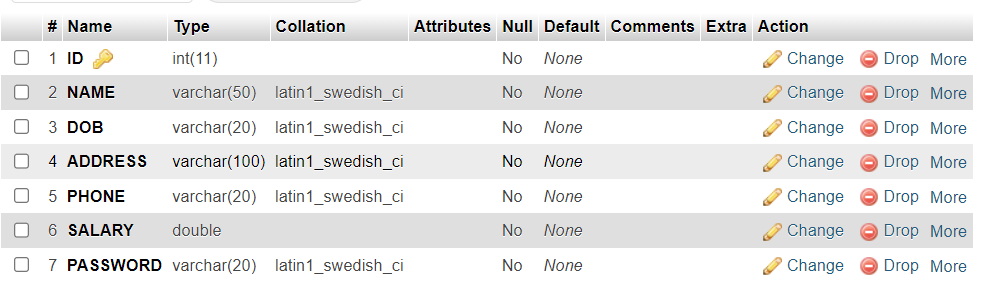
\includegraphics[width=1\textwidth]{users.png}
		\caption{users table}
		\label{table:users.png}
	\end{table}
\end{center}


\chapter{Screenshots}

Figure:\ref{fig:home page.png} shows the screenshot of Login page 
\begin{figure}[h]
 \centering
 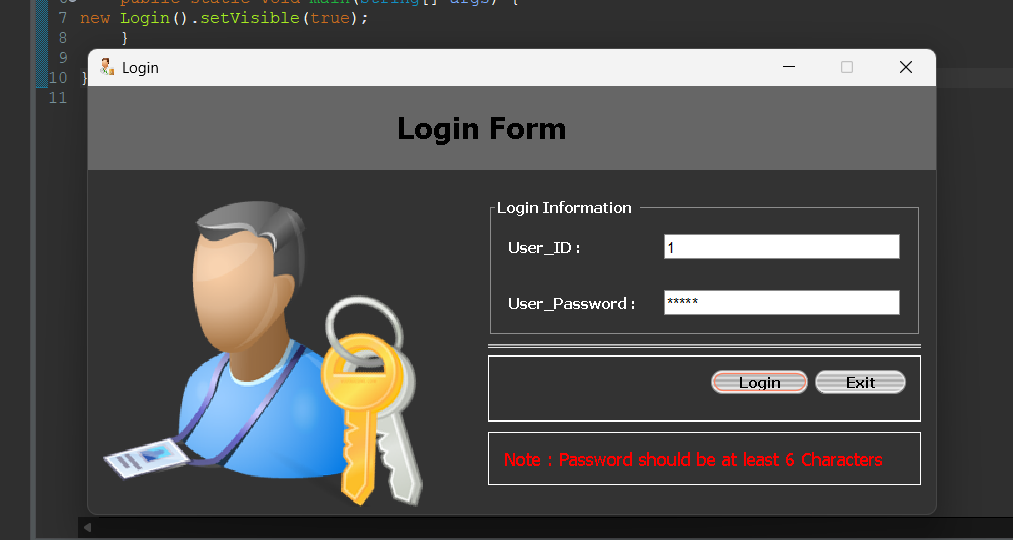
\includegraphics[width=0.75\textwidth]{home page.png}
 \caption{Login Page}
 \label{fig:home page.png}
\end{figure}

Figure:\ref{fig:2.png} shows the screenshot of home page
\begin{figure}[h]
 \centering
 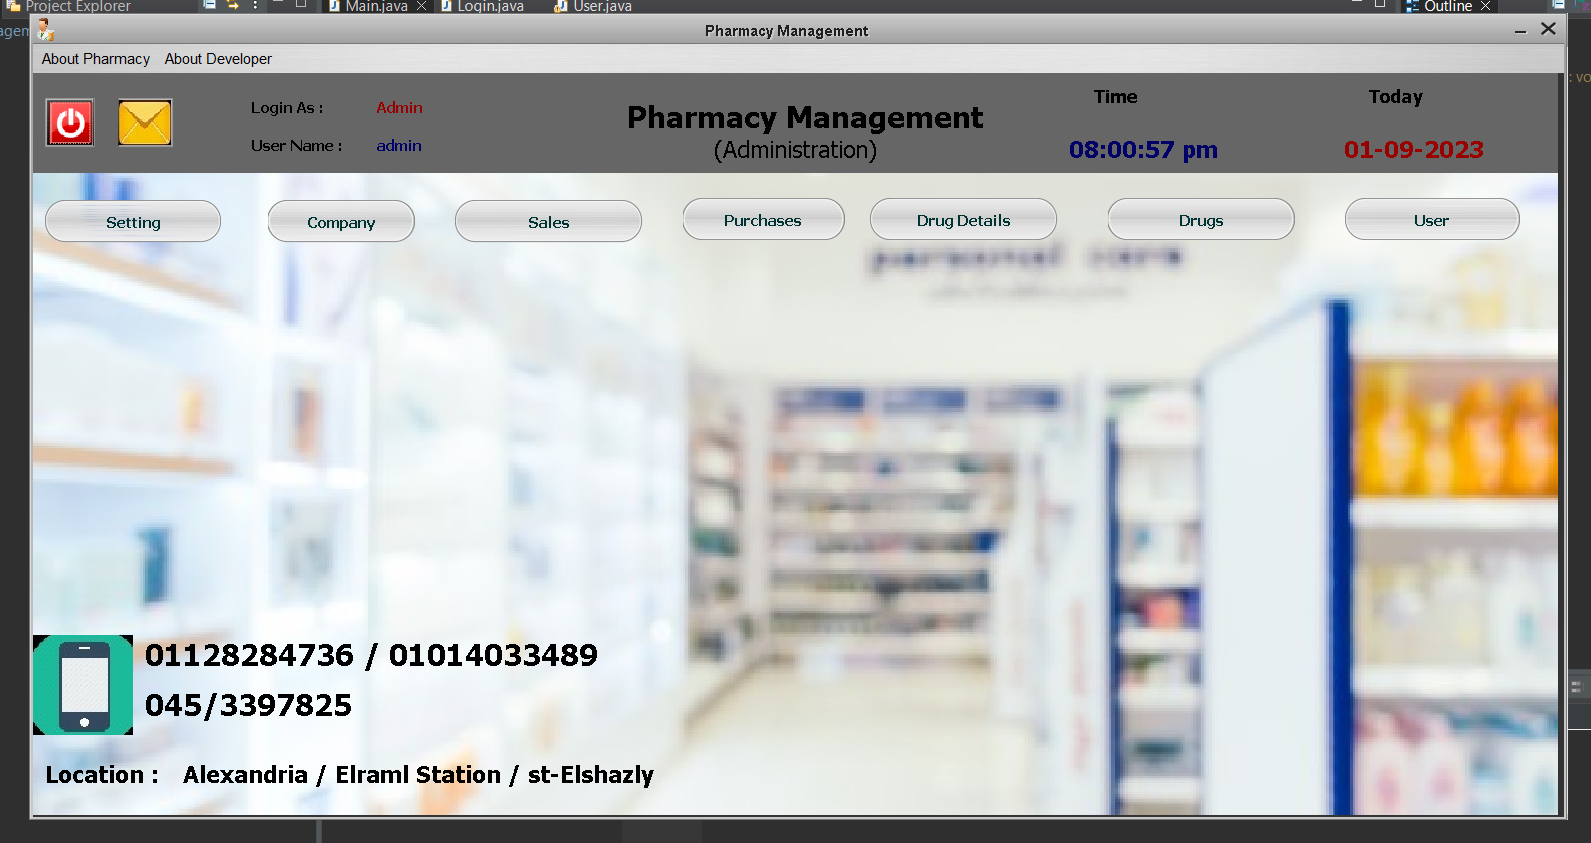
\includegraphics[width=0.75\textwidth]{2.png}
 \caption{admin home Page}
 \label{fig:2.png}
\end{figure}
\newpage
Figure:\ref{fig:druglist.png} shows the screenshot of drug list
\begin{figure}[h]
	\centering
	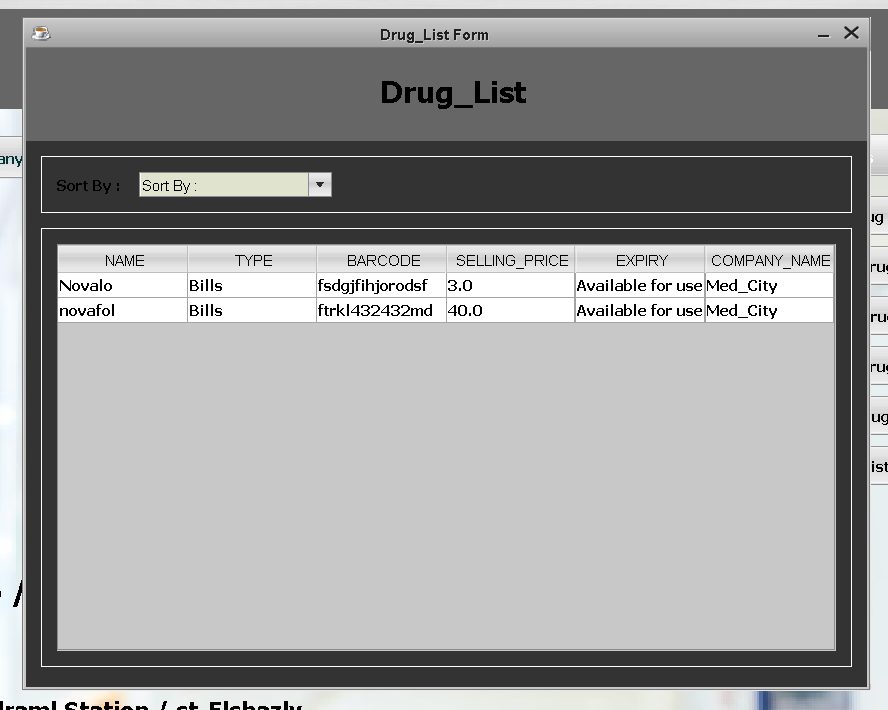
\includegraphics[width=0.6\textwidth]{druglist.png}
	\caption{drug list}
	\label{fig:druglist.png}
\end{figure}

Figure:\ref{fig:userinfo.png} shows the screenshot of user info
\begin{figure}[h]
	\centering
	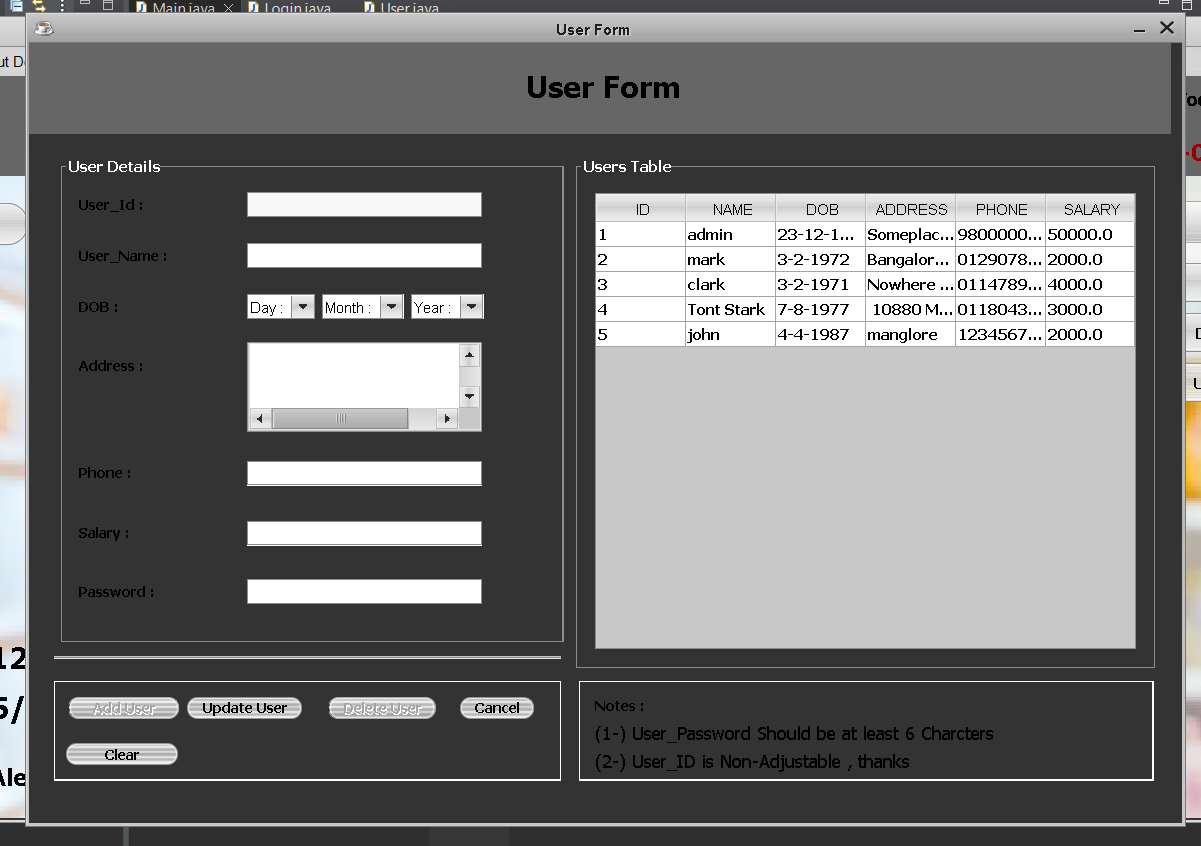
\includegraphics[width=0.6\textwidth]{userinfo.png}
	\caption{user info}
	\label{fig:userinfo.png}
\end{figure}
\newpage
Figure:\ref{fig:dealslist.png} shows the screenshot of deals list
\begin{figure}[h]
	\centering
	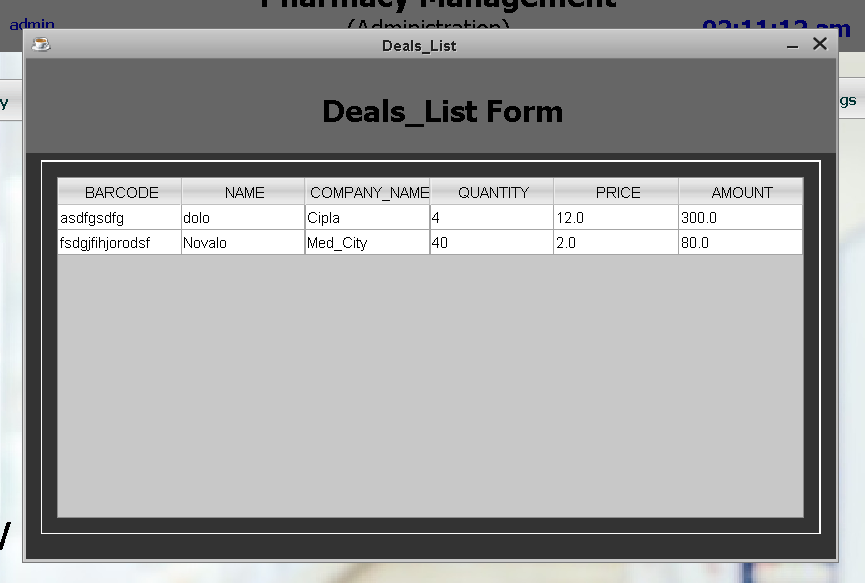
\includegraphics[width=0.75\textwidth]{dealslist.png}
	\caption{deals list}
	\label{fig:dealslist.png}
\end{figure}

\chapter{Conclusion and Future Scope}

\textbf{Conclusion} 
\begin{itemize}
 \item {Detailed information gathering has to be done. Without that, the purpose for using the software won't be satisfied properly.}
 \item {Implementing the software requires a change in business practices.}
 \item{Efficient organization of all knowledge and easy retrieval of information is possible.}
 \item{It leads to ease in functioning of business processes}
\end{itemize}
\textbf{Future Scope} 
\begin{itemize}
 \item {In this project, we can also include Bar code using bar code reader which will detect the expiry date and other related information. }
 \item {Project can be made more robust by adding bio-metric verification. }
 \item{There is also scope to expand by implementing newer technologies like AI,cloud etc.}
\end{itemize}

\begin{thebibliography}{7}
\addcontentsline{toc}{chapter}{References}
\bibitem{texbook}
Ramez Elmsari Shamkant and B.Navathe  \emph{e “Database System Models, Languages Design and Application Programming”},Pearson 7th Edition 2017.

\bibitem{texbook}
 Ramakrishna and Gehrke \emph{Database Management Systems}, McGraw Hill 3rd Edition 2014.

\bibitem{sql}
  \href{https://docs.oracle.com/en-us/iaas/mysql-database/doc/getting-started.html}{\emph{MySQL Documentation}}
 
 \bibitem{youtube}
 \href{www.youtube.com}{\emph{Youtube}}
 
 \bibitem{google}
\href{www.google.com}{\emph{Google}}

\end{thebibliography}


\end{document}
